\documentclass[11pt,a4paper]{article}
\usepackage[a4paper]{geometry}
\usepackage[utf8]{inputenc}
\usepackage[english]{babel}
\usepackage{lipsum}
\usepackage{eurosym}
\usepackage{rotating}

\usepackage{amsmath, amssymb, amsfonts, amsthm, mathtools}
% mathtools for: Aboxed (put box on last equation in align environment)
\usepackage{microtype} %improves the spacing between words and letters

\usepackage{lipsum}
\usepackage{threeparttable}
\usepackage{tabularx}
\usepackage{multirow}
\usepackage{booktabs}
\newcommand{\tabitem}{~~\llap{\textbullet}~~}
\usepackage{graphicx}
\graphicspath{ {./figures/} {./eps/}}
\usepackage{epsfig}
\usepackage{epstopdf}
\usepackage{verbatim}
\usepackage{textcomp}
\usepackage{tikz}
\usetikzlibrary{shapes,arrows}

\geometry{vmargin={2cm, 2cm}}
% Default fixed font does not support bold face
\DeclareFixedFont{\ttb}{T1}{txtt}{bx}{n}{12} % for bold
\DeclareFixedFont{\ttm}{T1}{txtt}{m}{n}{12}  % for normal

%%%%%%%%%%%%%%%%%%%%%%%%%%%%%%%%%%%%%%%%%%%%%%%%%%
%% COLOR DEFINITIONS
%%%%%%%%%%%%%%%%%%%%%%%%%%%%%%%%%%%%%%%%%%%%%%%%%%
 % Enabling mixing colors and color's call by 'svgnames'
%%%%%%%%%%%%%%%%%%%%%%%%%%%%%%%%%%%%%%%%%%%%%%%%%%
\definecolor{MyColor1}{HTML}{CC0000} %mix personal color
\newcommand{\textb}{\color{Black} \usefont{OT1}{lmss}{m}{n}}
\newcommand{\blue}{\color{MyColor1} \usefont{OT1}{lmss}{m}{n}}
\newcommand{\blueb}{\color{MyColor1} \usefont{OT1}{lmss}{b}{n}}
\newcommand{\red}{\color{LightCoral} \usefont{OT1}{lmss}{m}{n}}
\newcommand{\green}{\color{Turquoise} \usefont{OT1}{lmss}{m}{n}}
%%%%%%%%%%%%%%%%%%%%%%%%%%%%%%%%%%%%%%%%%%%%%%%%%%

%%%%%%%%%%%%%%%%%%%%%%%%%%%%%%%%%%%%%%%%%%%%%%%%%%
%% Scala coloring settings
%%%%%%%%%%%%%%%%%%%%%%%%%%%%%%%%%%%%%%%%%%%%%%%%%%
% "define" Scala
\usepackage{listings}
\usepackage{xcolor}
\lstset{escapeinside={<@}{@>}}
\definecolor{deepblue}{rgb}{0,0,0.5}
\definecolor{deepred}{rgb}{0.6,0,0}
\definecolor{deepgreen}{rgb}{0,0.5,0}

% Python style for highlighting
\newcommand\pythonstyle{\lstset{
language=Python,
basicstyle=\ttm,
otherkeywords={self},             % Add keywords here
keywordstyle=\ttb\color{deepblue},
emph={MyClass,__init__},          % Custom highlighting
emphstyle=\ttb\color{deepred},    % Custom highlighting style
stringstyle=\color{deepgreen},
frame=tb,                         % Any extra options here
showstringspaces=false            % 
}}

% Python environment
\lstnewenvironment{python}[1][]
{
\pythonstyle
\lstset{#1}
}
{}

% Python for external files
\newcommand\pythonexternal[2][]{{
\pythonstyle
\lstinputlisting[#1]{#2}}}

% Python for inline
\newcommand\pythoninline[1]{{\pythonstyle\lstinline!#1!}}


%%%%%%%%%%%%%%%%%%%%%%%%%%%%%%%%%%%%%%%%%%%%%%%%%%
%% FONTS AND COLORS
%%%%%%%%%%%%%%%%%%%%%%%%%%%%%%%%%%%%%%%%%%%%%%%%%%
%		SECTIONS
%%%%%%%%%%%%%%%%%%%%%%%%%%%%%%%%%%%%%%%%%%%%%%%%%%
\usepackage{titlesec}
\usepackage{sectsty}
%%%%%%%%%%%%%%%%%%%%%%%%
%set section/subsections HEADINGS font and color
\sectionfont{\color{MyColor1}}  % sets colour of sections
\subsectionfont{\color{MyColor1}}  % sets colour of sections

%set section enumerator to arabic number (see footnotes markings alternatives)
\renewcommand\thesection{Exercise \arabic{section}} %define sections numbering
\renewcommand\thesubsection{\thesection.\arabic{subsection}} %subsec.num.

%define new section style
\newcommand{\mysection}{
\titleformat{\section} [runin] {\usefont{OT1}{lmss}{b}{n}\color{MyColor1}}
{\thesection} {3pt} {} }

%%%%%%%%%%%%%%%%%%%%%%%%%%%%%%%%%%%%%%%%%%%%%%%%%%
%		CAPTIONS
%%%%%%%%%%%%%%%%%%%%%%%%%%%%%%%%%%%%%%%%%%%%%%%%%%
\usepackage{caption}
\usepackage{subcaption}
%%%%%%%%%%%%%%%%%%%%%%%%
\captionsetup[figure]{labelfont={color=MyColor1}}

%%%%%%%%%%%%%%%%%%%%%%%%%%%%%%%%%%%%%%%%%%%%%%%%%%
%		!!!EQUATION (ARRAY) --> USING ALIGN INSTEAD
%%%%%%%%%%%%%%%%%%%%%%%%%%%%%%%%%%%%%%%%%%%%%%%%%%
%using amsmath package to redefine eq. numeration (1.1, 1.2, ...)
%%%%%%%%%%%%%%%%%%%%%%%%
\renewcommand{\theequation}{\arabic{equation}}

%set box background to grey in align environment
\usepackage{etoolbox}% http://ctan.org/pkg/etoolbox
\makeatletter
\patchcmd{\@Aboxed}{\boxed{#1#2}}{\colorbox{black!15}{$#1#2$}}{}{}%
\patchcmd{\@boxed}{\boxed{#1#2}}{\colorbox{black!15}{$#1#2$}}{}{}%
\makeatother
%%%%%%%%%%%%%%%%%%%%%%%%%%%%%%%%%%%%%%%%%%%%%%%%%%

\newcommand{\DP}[1]{\textcolor{blue}{\textbf{(DP says: #1)}}}

\makeatletter
\let\reftagform@=\tagform@
\def\tagform@#1{\maketag@@@{(\ignorespaces\textcolor{red}{#1}\unskip\@@italiccorr)}}
\renewcommand{\eqref}[1]{\textup{\reftagform@{\ref{#1}}}}
\makeatother
\usepackage[hidelinks]{hyperref}

%% LISTS CONFIGURATION %%
\usepackage{enumitem}
\setlist[enumerate,1]{start=0}
\renewcommand{\labelenumii}{\theenumii}
\renewcommand{\theenumii}{\theenumi.\arabic{enumii}.}

\usepackage[acronym]{glossaries}
\newacronym{ci}{CI}{Confidence Interval}
\newacronym{pi}{PI}{Prediction Interval}
\newacronym{lcg}{LCG}{Linear Congruence Generator}

%%%%%%%%%%%%%%%%%%%%%%%%%%%%%%%%%%%%%%%%%%%%%%%%%%
%% PREPARE TITLE
%%%%%%%%%%%%%%%%%%%%%%%%%%%%%%%%%%%%%%%%%%%%%%%%%%
\title{\blue Network analysis and simulation\\ Homework 1}
\author{Davide Peron}
\date{}
%%%%%%%%%%%%%%%%%%%%%%%%%%%%%%%%%%%%%%%%%%%%%%%%%%

\begin{document}
\maketitle
\section{}
In \autoref{fig:6_5a}, \autoref{fig:6_5b}, \autoref{fig:6_5c}, \autoref{fig:6_7a} and \autoref{fig:6_7b}, the behavior of a \gls{lcg} has been studied. In the last two figures, the two \textit{non-standard} distributions have been taken in account. In \autoref{fig:6_10a} the distribution is
$$
f_Y(y) = K\frac{sin^2(y)}{y^2}\mathbf{1}_{\{-a \le y \le a\}}
$$
with $a=10$, while in \autoref{fig:6_10b} there are a set of sample of the random vector $(X_1, X_2)$ with a density proportional to $|X_1 - X_2|$.

In the follow the said figures are reported.

\begin{figure}[ht]
	\centering
	\begin{minipage}{0.45\textwidth}
		\centering
		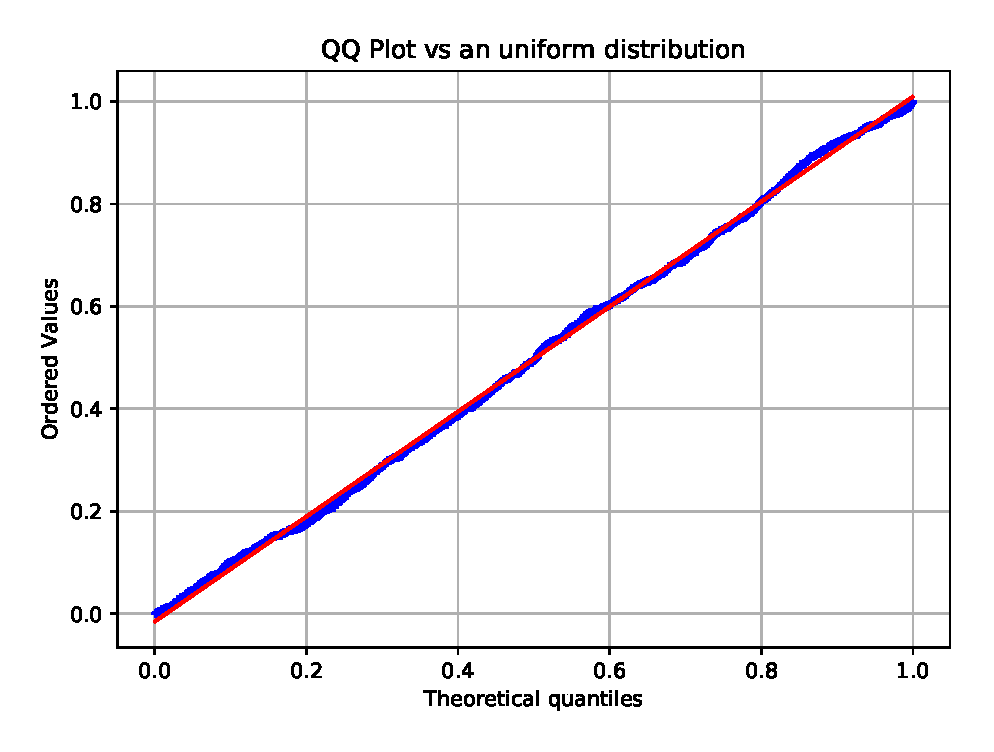
\includegraphics[width=\textwidth]{fig-6_5a}
		\caption{QQPlot of the \gls{lcg} versus a uniform distribution (Figure 6.5a)}
		\label{fig:6_5a}
	\end{minipage}
	\begin{minipage}{0.45\textwidth}
		\centering
		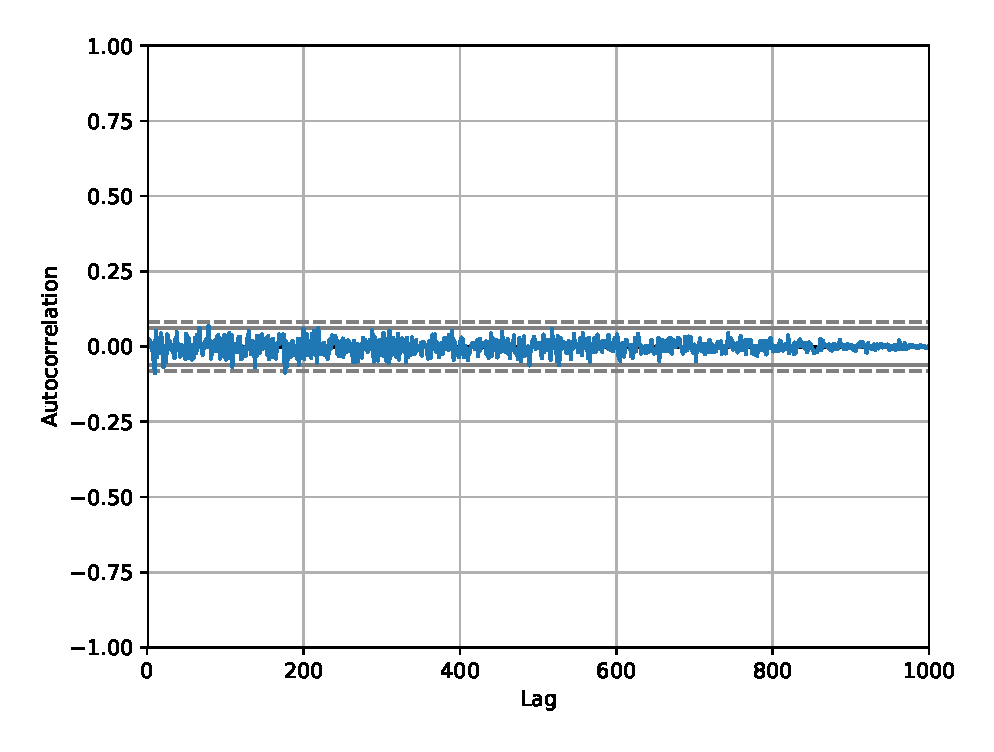
\includegraphics[width=\textwidth]{fig-6_5b}
		\caption{Autocorrelation of the \gls{lcg} (Figure 6.5b)}
		\label{fig:6_5b}
	\end{minipage}
\end{figure}

\begin{figure}[ht]
  \centering
  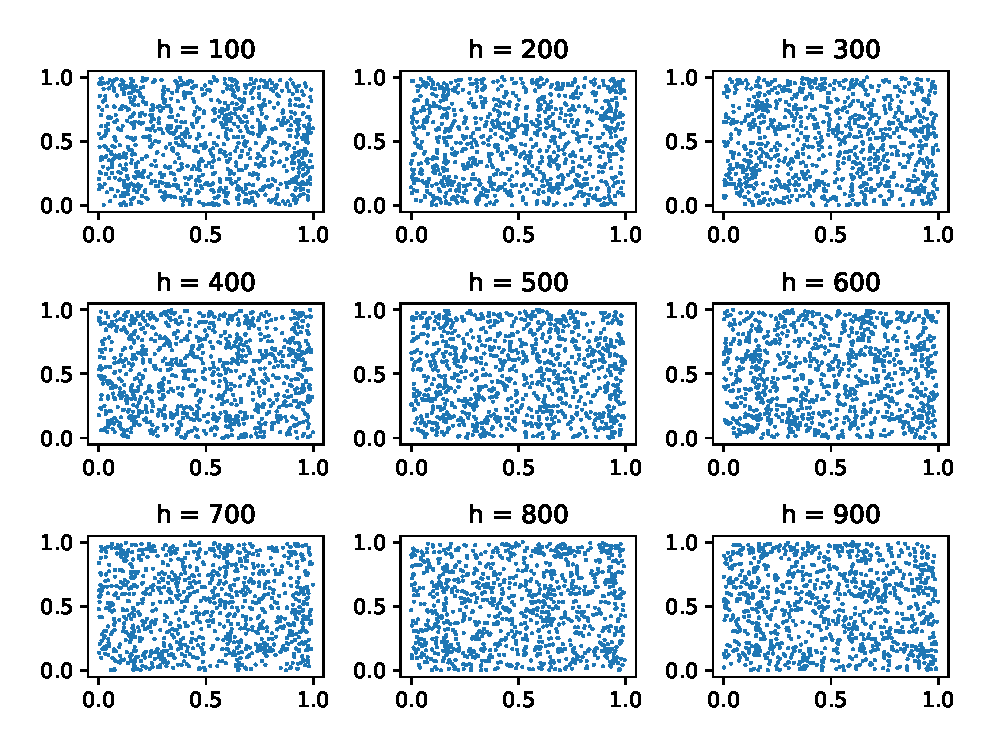
\includegraphics[width=0.9\textwidth]{fig-6_5c}
  \caption{Lag plots (Figure 6.5c)}
  \label{fig:6_5c}
\end{figure}

\begin{figure}[ht]
	\centering
	\begin{minipage}{0.45\textwidth}
		\centering
		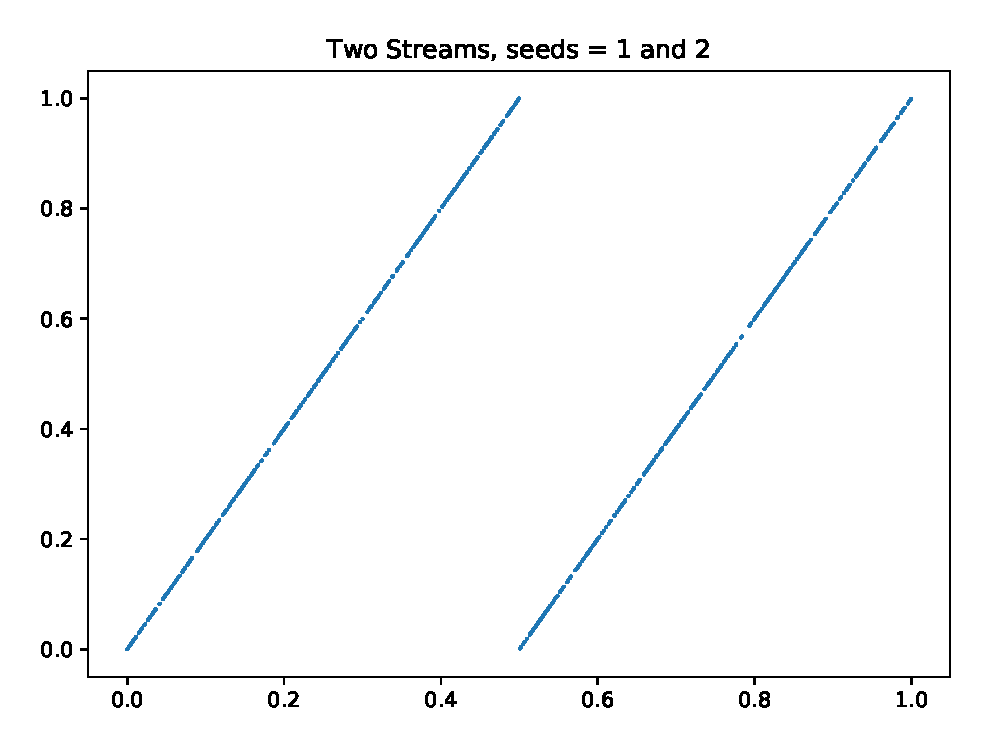
\includegraphics[width=\textwidth]{fig-6_7a}
		\caption{Behavior of two parallel stream using seed $s=1$ and $s=2$ (Figure 6.7a) }
		\label{fig:6_7a}
	\end{minipage}
	\begin{minipage}{0.45\textwidth}
		\centering
		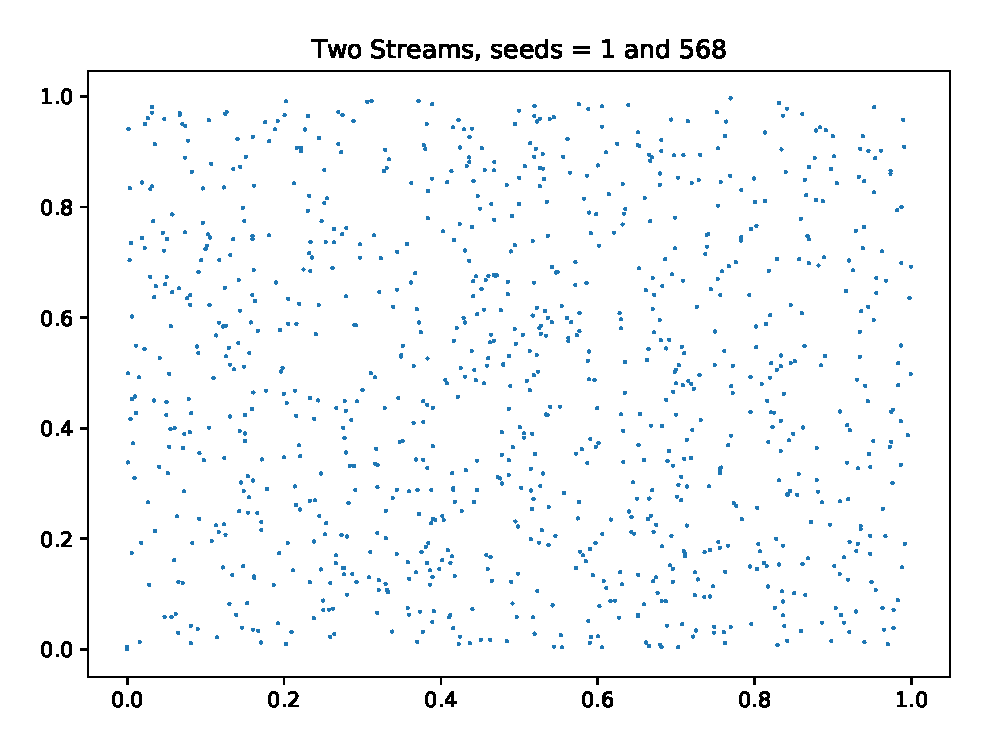
\includegraphics[width=\textwidth]{fig-6_7b}
		\caption{Behavior of two parallel stream using seed $s=1$ and $s=568$ (Figure 6.7b)}
		\label{fig:6_7b}
	\end{minipage}
\end{figure}

\begin{figure}[ht]
	\centering
	\begin{minipage}{0.45\textwidth}
		\centering
		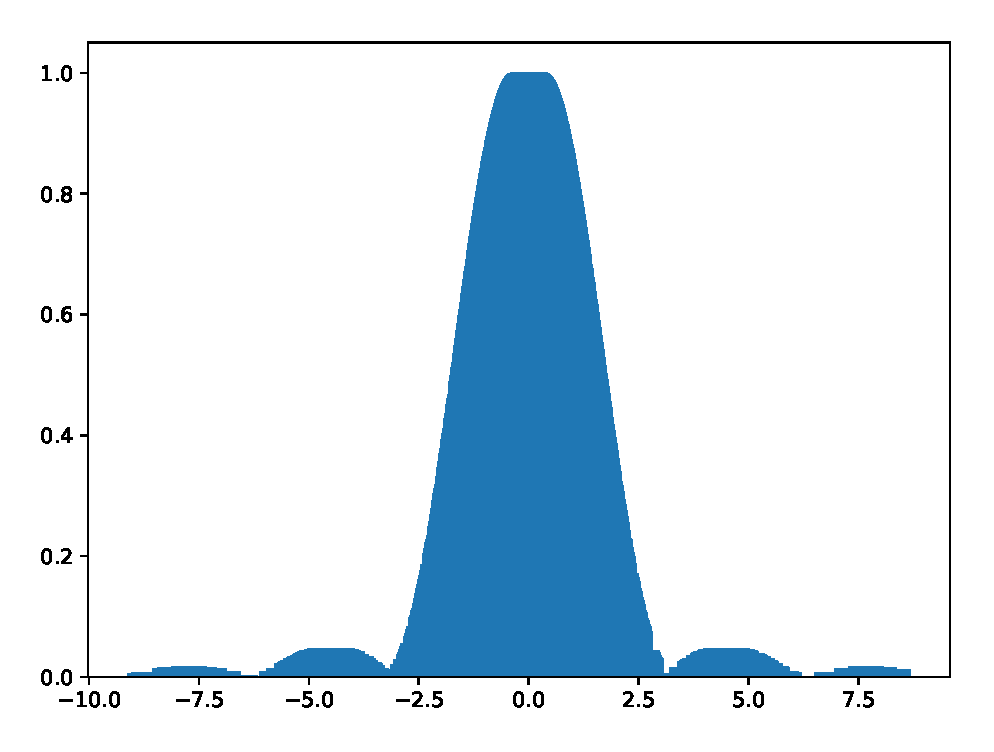
\includegraphics[width=\textwidth]{fig-6_10a}
		\caption{Histograms of a set of sample from the first \textit{weird} distribution (Figure 6.10a)}
		\label{fig:6_10a}
	\end{minipage}
	\begin{minipage}{0.45\textwidth}
		\centering
		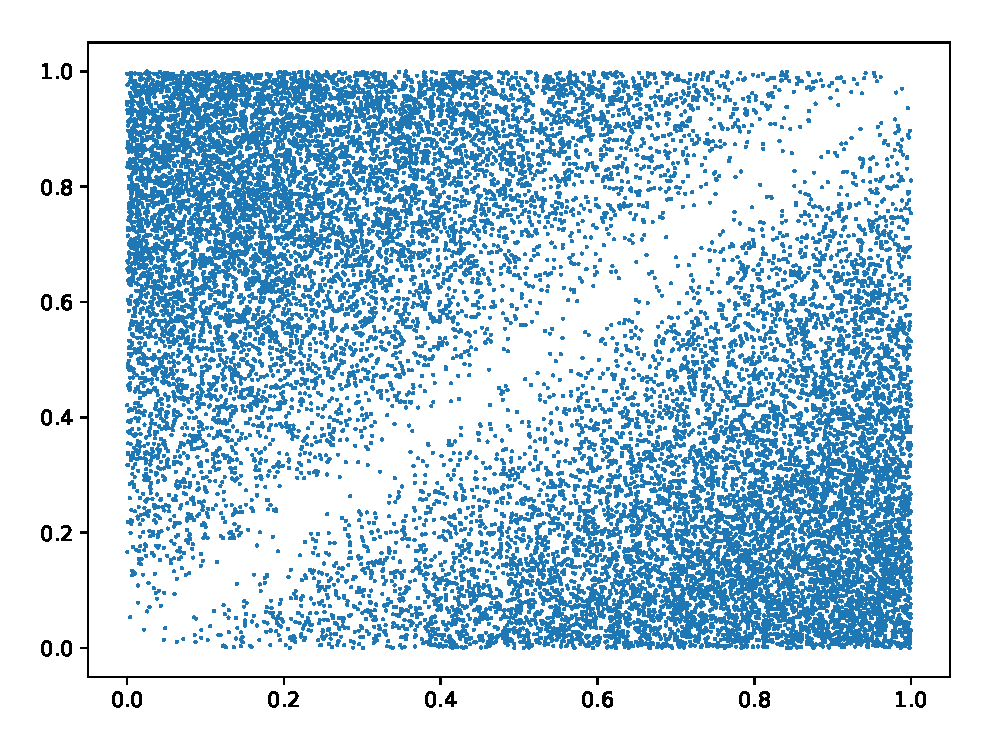
\includegraphics[width=\textwidth]{fig-6_10b}
		\caption{Set of sample from the second \textit{weird} distribution (Figure 6.10b)}
		\label{fig:6_10b}
	\end{minipage}
\end{figure}

\newpage
\section{}
Trying to generate a set Binomial random variables $B(n,p)$ with $n=50$ and $p=0.5$, we can see that the fastest approach is the CDF inversion technique, although extracting $n$ Bernoulli rvs is much faster than the Geometric method.
In the follow, the three different implementations are presented.

The first method inplemented is the one of the CDF inversion.
\begin{python}
  # With CDF inversion

X_CDF = []
F_CDF = []
start = time.time()
c = theta/(1-theta)
for _ in range(0,n_rvs):
    pr = (1-theta)**n
    u = np.random.rand()
    i = 0
    F = pr
    while u >= F:
        pr *= c*(n-i)/(i+1)
        F += pr
        i += 1
    X_CDF.append(i)
    F_CDF.append(F)
    mean_CDF += i
end = time.time()
time_CDF = end - start
\end{python}

A Binomial Random Variable can also be created drawing $n$ Bernoulli rvs and counting the successes.
\begin{python}
  # Drawing n Bernoulli rvs
start = time.time()

for _ in range(0,n_rvs):
    X_bernoulli = 0
    for i in range(0,50):
        u = np.random.rand()
        if u > 0.5: #Success
            X_bernoulli += 1
    mean_bernoulli += X_bernoulli
end = time.time()
time_bernoulli = end - start
\end{python}

A method to avoid to draw $n$ Bernoulli rvs is to count how much geometric fits into $n$ trials
\DP{Qui è da rivedere}, although this approach is the one that requires less operations, is the slower one, probably due to the computational complexity of the $log$ function.

\begin{python}
  # Using Geometric Distribution

start = time.time()
for _ in range(0,n_rvs):
    isFinished = False
    X_geometric = 0
    count = 0
    while not isFinished:
        u = np.random.rand()
        X_geometric += np.floor(np.log(u)/np.log(1-theta)) + 1
        if X_geometric >= n :
            isFinished = True
        if X_geometric <= n:
            count += 1
    mean_geometric += count
end = time.time()
time_geometric = end - start
\end{python}

\section{}
Trying to generate a set Poisson random variables $P(\lambda)$ with $\lambda = 5$, we can see that, also in this case, the fastest method is the CDF inversion technique, immediately followed by the Uniform rvs method and the Exponential one.
In the follow, the three different implementations are presented.

The first method inplemented is the one of the CDF inversion.
\begin{python}
#CDF Inversion
mean_CDF = 0
start = time.time()
for k in range(0,n_vars):
    u = np.random.rand()
    i = 0
    p = math.exp(-lambda_par)
    F = p
    while u >= F:
        p *= lambda_par/(i+1)
        F += p
        i += 1
    mean_CDF += i

mean_CDF /= n_vars
end = time.time()
time_CDF = end - start
\end{python}

A Poisson Random Variable can also be created counting the number of exponential rvs that you can draw until their sum is less than $1$.
\begin{python}
#Sum of exponentials
mean_exp = 0
start = time.time()
for i in range(0,n_vars):
    n_exp = 0
    sum = 0
    while sum <= 1:
        sum += -math.log(np.random.rand())/lambda_par
        n_exp += 1
    mean_exp += n_exp - 1

mean_exp /= n_vars
end = time.time()
time_exp = end - start
\end{python}

The last method is using uniforms as long as their product is greater than $e^{-\lambda}$.
\begin{python}
  #Product of uniforms
mean_unif = 0
start = time.time()
for i in range(0,n_vars):
    rv = 1
    count = 0
    while rv > math.exp(-lambda_par):
        rv *= np.random.rand()
        count += 1
    mean_unif += count - 1

mean_unif /= n_vars
end = time.time()
time_unif = end - start
  \end{python}
\end{document}